\documentclass[aspectratio=169]{beamer}
\usetheme{metropolis}
\title{E4E Drill Press Fundamentals Workshop}
\institute{Engineers for Exploration, UC San Diego}
\date{December 7, 2023}
\logo{
\includegraphics[height=.65cm]{e4e_logo_350x136.png}}
\setbeamertemplate{caption}[numbered]

\usepackage{graphicx}
\usepackage{hyperref}
\usepackage{booktabs}

\begin{document}
\maketitle
\begin{frame}{Safety Considerations}
    \begin{enumerate}
        \item Where is the stored energy?
        \item Where is the exposed energy?
        \item How can the energy be transferred?
    \end{enumerate}
\end{frame}
\begin{frame}{What is on a Drill Press?}
    \centering
    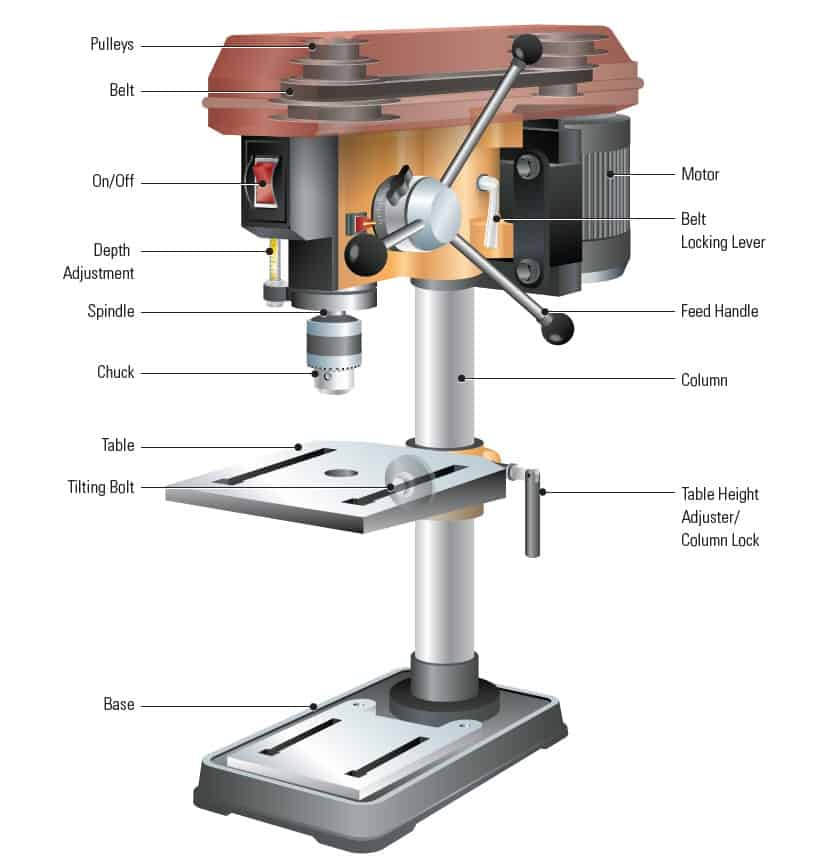
\includegraphics[height=0.7\textheight]{drill_press_anatomy.jpg} \footnote{\url{https://canadianwoodworking.com/tools/drill-press/}}
\end{frame}
\begin{frame}{Layout}
    \begin{itemize}
        \item Scribes
        \item Center Punches
        \item Layout Blacking
    \end{itemize}
\end{frame}
\begin{frame}{Drill Bit Anatomy}
    \centering
    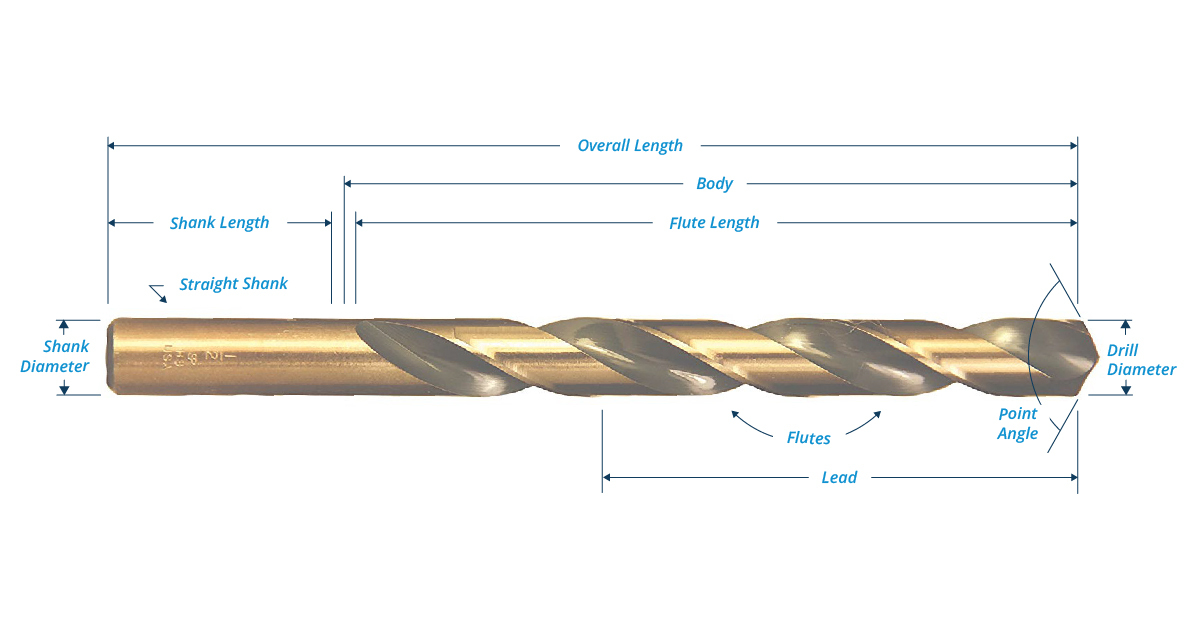
\includegraphics[height=0.7\textheight]{drill_bit_anatomy.jpg} \footnote{\url{https://www.xometry.com/resources/shop-tips/drill-bit-tips-tricks/}}
\end{frame}
\begin{frame}{Other Drill Press Cutters}
    \centering
    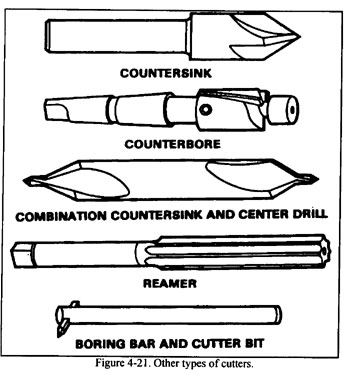
\includegraphics[height=0.7\textheight]{drill_press_tools.jpg} \footnote{\url{https://www.americanmachinetools.com/how_to_use_a_drill_press.htm}}
\end{frame}
\begin{frame}{Drill Bit Sizes}
    \begin{itemize}
        \item How much material to remove?
        \item How hard is the material?
        \item Wire/Letter/Fractional/Metric
    \end{itemize}
\end{frame}
\begin{frame}{Drill Press Speed}
    $$RPM = CS \times \frac{4}{D}$$
    \centering
    \begin{tabular}{@{}lll@{}}
        \toprule
        Material                      & Drilling Feet/Minute & Reaming Feet/Minute \\\midrule
        Carbon steels                 & 100 - 120            & 75 - 80               \\
        Carbon steels                 & 35 - 70              & 20 - 45               \\
        Alloy steels (resulfurized)   & 30 - 90              & 15 - 60               \\
        Stainless steels (Austenitic) & 50 - 55              & 30 - 35               \\
        Brass                         & 160 - 175            & 160 - 175             \\
        Bronze                        & 120 - 140            & 110 - 120             \\
        Wrought aluminum              & 350 - 400            & 350 - 400            \\ \bottomrule
    \end{tabular}
\end{frame}
\begin{frame}{Drill Chuck Anatomy}
    \centering
    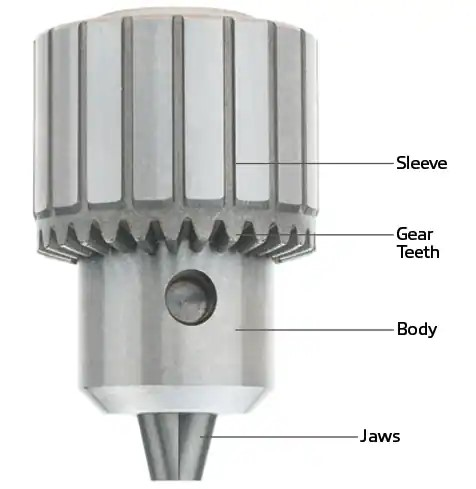
\includegraphics[height=0.7\textheight]{drill_chuck.jpg} \footnote{\url{https://www.mscdirect.com/basicsof/drill-chucks}}
\end{frame}
\begin{frame}{Workholding}
    \begin{columns}
        \begin{column}{0.5\textwidth}
            \centering
            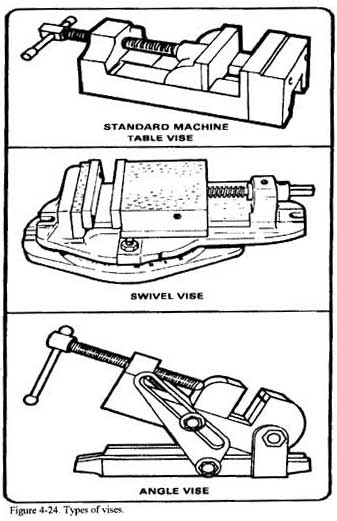
\includegraphics[height=0.7\textheight]{drill_vises.jpg}
        \end{column}
        \begin{column}{0.5\textwidth}
            \centering
            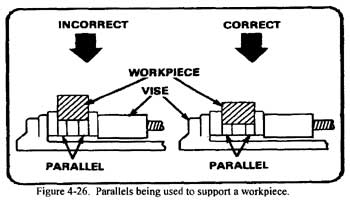
\includegraphics[width=0.9\linewidth]{vise_parallels.jpg} \footnote{\url{https://www.americanmachinetools.com/how_to_use_a_drill_press.htm}}
        \end{column}
    \end{columns}
\end{frame}
\begin{frame}{Cutting Fluids}
    \begin{enumerate}
        \item Cooling
        \item Lubrication
        \item Chip Evacuation
    \end{enumerate}
\end{frame}
\begin{frame}{Feed Speed}
    \begin{enumerate}
        \item Chip Loading
        \item Chip Sizes
        \item Machine Power
    \end{enumerate}
\end{frame}
\begin{frame}{Permissible Materials}
    \begin{enumerate}
        \item Plastics
        \item Wood
        \item Metals
    \end{enumerate}
\end{frame}
\begin{frame}{Maintenance}
    \begin{enumerate}
        \item Powertrain
        \item Cleaning
        \item Configuration
    \end{enumerate}
\end{frame}
\begin{frame}{Access Protocol}
    \begin{enumerate}
        \item LO/TO
        \item Cleanup
    \end{enumerate}
\end{frame}
\begin{frame}{Practical Exercise}
    \centering
    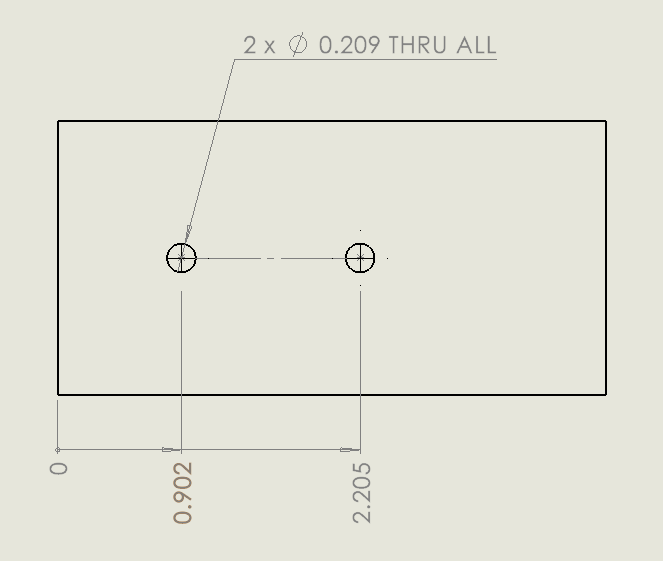
\includegraphics[height=0.7\textheight]{exercise1.png}
\end{frame}
\end{document}